\chapter{Музыкальные магазины}

%Эту главу я задумал, возвращаясь домой в такой ветер с дождем, что клонило к земле. Между тем было начало января 2014, без снега, мрачный день с тучами, более гожими для августовского неба. Сначала писать мне помешал стук в компьютере, я разобрал корпус, вынул винчестеры и вставил обратно, закрыл корпус, вспомнил, что забыл прикрутить один винтик, открыл корпус, поставил всё на место, закрыл, потом снова услышал стук, но возиться с этим дальше уже не было сил.

Музыкальными магазинами открываю особую часть книги – с воспоминаниями. Всё равно меня постоянно уносит в них, так лучше отвести им отдельное место, чем пускаться в плавание по морю памяти везде, где блажь найдет.

Под музыкальными магазинами подразумеваю такие, где продается музыка, а не инструменты. Века нынешнего я почти не буду касаться, ибо давно перестал покупать музыку. Чтобы легче было рассказывать, упорядочу повествование по времени, двигаясь от прошлого к настоящему.

Моя мама в середине 1970-х годов работала продавцом в отделе классической музыки магазина «Грампластинки», что на Красноармейской 4. Я там никогда не был. В нем торговали не только винилом, но и бобинами и входившими в моду аудиокассетами. %Также существовал отдел пластинок в «Нотах» на Крещатике.

Я помню, что до школы я слушал Beatles с маленьких пластинок – 17-сантиметровых «миньонов», где на обложке невесть зачем писали, что слова народные, а не Beatles. Слушал Африк Симона с голубой гибкой пластинки, Пугачову, Тыниса Мяги, Boney M, Simon and Garfunkel, какие-то сборники под названием «Звезды диско», но больше музыки любил разные звуковые спектакли, которых в Советском Союзе выпускали для детей очень много. «Велунд», «Песнь о Роланде», «Король Артур и рыцари круглого стола», всякие веселые сказки, серия «КОАПП» и прочее. Это я крутил, до того как папа подарил «Радиотехнику», проигрыватель «Юность». Такой чемоданчик, открываешь – в крышке динамик, а внизу вертушка. Любимой моей пластинкой была «Американская сельская музыка», которую я запилил за несколько лет частого прослушивания. До сих пор помню оттуда мелодии и бессвязные слова – не зная еще английского, я повторял набор звуков.

Пластинки мы покупали в двух магазинах. Первый, «Мелодия», был к нашему дому на Бастионной ближе. Он располагался на бульваре Дружбы Народов, 14 – угловой дом рядом с пустырем – и напротив через дорогу такой же пустырь. Сейчас тот, через улицу, обнесен забором, а на месте пустыря около магазина (квадрат между улицами Дружбы Народов, Товарной и Чешской) построили супермаркет «Новус» и какой-то еще огромный дом, хотя еще с конца советских времен там собирались строить метро, и метростроевская ограда долго охраняла местность. В помещении «Мелодии», зимой 2015 года – отделение «Новой почты».

К «Мелодии» с Бастионной надо идти пешком, и проще было добраться на 14 троллейбусе\footnote{Он тогда ходил от ботсада на Зверинце до Бессарабки.} до «Подарочного» на бульваре Леси Украинки. Там были отделы с игрушками и пластинками.

Я бродил в тех краях последний раз, когда застраивали овраг в Клове, между Леси Украинки, 9 и библиотекой Щедрина. Помню, как в детстве ходил по тропе над оврагом, где из темноты поднимались могучие деревья. Вдоль тропы один за другим следовали белые столбики с красными полосками. А в 21 веке деревья подчистую спилили, склон раскопали и укрепили, да соорудили дома. Не знаю, кто нас надоумил – в восьмидесятых, на той тропе, мы с бабушкой собирали шампиньоны. Мама когда узнала, то запретила это делать. Один раз, я перочинным ножиком выковырял над обрывом Клова целую грибницу, 15 штук грибов!

«Подарочный» занимал два этажа панельного, высотного по тем временам дома сразу за библиотекой. Мы выходили на остановке около библиотеки и немного спускались к «Подарочному». В него можно было войти с одной стороны, пройти насквозь и покинуть в конце, ниже. А дальше находился еще один интересный магазин – «Дом радио». Сейчас это номера 5 и 3. Чуть спустись, и садишься на трамвай по улице Мечникова. На былой остановке ныне торчит небоскреб. Давно, давно не звенит трамвай на Клове и Саксаганского.

В «Подарочном» отдел пластинок был последним по счету, на первом этаже. Еще там продавались, кроме игрушек, разная парфюмерия, модели машинок, часы, брошки-сережки, небольшие картины в рамках, вышивки – это я уже смутно помню, потому что мне нужны были только игрушки и пластинки. В 90-х годах, не доходя до отдела пластинок появился еще один, с игровыми приставками «Денди» и «Сега», и картриджами к ним. Популярного тогда обмена картриджей в «Подарочном» вроде не было, иначе мы с братом не ездили бы за обменом к черту на Кулички, в конец бульвара Лепсе или на Кардачи.

Когда я пошел в школу, на Печерске построили «Торговый центр». Навскидку не скажу улиц – я могу туда дойти, наверное не узнаю, всё изменилось. Быть может улица Суворова? Мы туда ехали на 62-м автобусе, выходили почти напротив проходной «Арсенала», на Московской, и пешком топали вглубь кварталов из невысоких старых зданий и белых шестнадцатиэтажек. По пути, еще на Московской улице, первый этаж жилого дома занимал хороший книжный магазин.

«Торговый центр», как сейчас понимаю, чем-то походил на современные супермаркеты, но без такого пространственного размаха, да с правильными советскими ценами. На первом этаже были продукты и, около лестницы, отдел пластинок. Там то с папой, то с мамой мы покупали выпуски появившейся тогда серии «Архив популярной музыки», которую составлял, как я проведал позже, известный по эпохе видеотек переводчик Володарский. 

В этой серии выходили лучшие записи Led Zeppelin, Deep Purple, словом, рока 70-х. Попутно стали продаваться пластинки без серий. Emerson, Lake and Palmer. Black Sabbath понравился мне песней «Iron Man» – там в самом начале роботический голос протяжно произносит: «ай эм ааайрон мээээн». Большим счастьем счел купить в серебристом конверте, болгарскую пластинку Майкла Джексона, но песни на ней эпохи «Триллера» показались мне слащавыми. Наверное несколько раньше того времени я много слушал Modern Talking, две известные их песни.

В первых классах школы ходил слух о некоем жанре офигезной музыки, назывался он «хэви мэтал». Нечто темное и запретное. Никто толком не знал, как оно звучит, но все старательно и значимо выводили на промокашках или, с особой смелостью – прямо на обложках тетрадей – вот такое:

\begin{center}

\includegraphics[width=0.20\linewidth]{chast-vosp/musmags/hmr.pdf}
\end{center}

Что означало «Хэви метал рок». Но кое-кто шел дальше и рисовал:

\begin{center}

\includegraphics[width=0.20\linewidth]{chast-vosp/musmags/hmp.pdf}
\end{center}

Его спрашивали – что это значит? «А это – хэви метал пэр». Что за «пэр» такой, до сих пор понять не могу. Еще знали названия разных групп и тоже их писали, вроде AC/DC, Metallica и Kiss.

А была училка молодая рисования, она же что-то по пионерским делам, увидела в тетрадке Яши Старосельского это «Kiss», и стала кричать – а ты знаешь, что они фашисты? Надо сказать, что буквам «SS» в логотипе Kiss в самом деле придается печально известное начертание, впрочем древние руны не виноваты, что их использовали гитлеровцы. Но в Германии поныне логотип группы Kiss печатают иначе, чем в остальных странах. Во избежание сходства. Не знаю, что побудило основателей группы, евреев Джина Симмонса и Пола Стэнли, придумать такую мороку.

Сам по себе рок в школе воспринимался нормально. Учитель английского языка, Федор Витальевич, как-то сказал нам – принесите свои любимые пластинки на английском, будем слушать и разбирать тексты песен. Я притащил кажется сборник Deep Purple. Было утро моего внутреннего торжества! Даже жарко стало, когда шел по классу к проигрывателю и ставил «свою» музыку.

Кроме отдела пластинок, «Торговый центр» был еще знаменит французскими батонами, которыми пахло еще по приближении к нему. В Советском Союзе делали очень вкусный хлеб, гораздо лучше нынешнего, но длинных горячих батонов не продавали. А тут появились. Их выпекали на втором этаже, и вывозили на черной стойке, где каждый батон покоился в эдаком ложе из мелкой металлической сетки. Другая, опустошенная стойка, отправлялась в печь с новым тестом. Стойка была за стеной с окошком. Мимо стены в полроста ограда. Заходишь за нее в очередь, берешь сколько нужно батонов – обычно мы брали два – и следуешь к кассе.

Горячие! С хрустящей тонкой корочкой! Соленые внутри! Ходили слухи, что внутрь батонов кладется сыр. Половину батона я уминал по пути к автобусу, еще половину – пока ехали домой. Остывший батон тоже был вкусен, хотя терял от увлажнения хрусткость корки. Редко французский хлеб переживал ночь. А когда ехали в автобусе, мне нравилось умозрительно измерять, как несколько батонов может во мне поместиться.

Относительно неподалеку от Торгового центра, около старинного Печерского базара – описанного у Лескова в «Печерских антиках» – примерно в то же время, раньше или позже, построили еще один магазин вроде супермаркета, только другой архитектуры, круглый, если глядеть на него сверху. 

Его мы тоже посещали, внутри была одна особенность – круглые пышки, выпекаемые прямо на месте, на первом этаже. Покупая, мы всегда просили, чтобы их не посыпали сахарной пудрой. Наверное плохо, что я не описываю что было в районе вокруг, ведь сейчас там всё изменилось, выросли огромные дома, старое разрушено, а я просто не помню ничего, кроме этого «Универсама» да хилого базара, прилепившегося сбоку. 

У меня в памяти возникают игрушки на втором этаже, продуктовый отдел с тележками на первом, бетонные плиты у входа, а на рынке – редис и клубника, да картошка. Самый близкий к нам базар. Был впрочем еще ближе, махонький, на Пятачке, в удолье на пересечении Бастионной и Киквидзе. 

Пора отлепиться мне от пышек и батонов. Прошло время, в начале 90-х у меня появился магнитофон-приста\-вка «Радиотехника», усилителем для коего служил упомянутый ранее проигрыватель. Тогдашняя советская техника была оснащена разъемом «УНИВ», то есть универсальным. Через него можно было подключить магнитофон к усилку, телевизор к магнитофону и так далее.

\begin{center}
\includegraphics[width=\linewidth]{chast-vosp/musmags/\myimgprefix IMG_4279.JPG}
\end{center}

«Радиотехника» у меня до сих жива и работает. Это замечательный аппарат с выдвижной кареткой для кассеты, индикатором громкости и расхода ленты, системой шумопонижения, памятью (выключение в нужном месте по счетчику оборотов) и уймой других полезностей. Мне нравились переносные магнитофоны, папа же считал, что музыку надо слушать «на стационаре», и признаю, что качество звучания связки магнитофон + усилок и две хорошие колонки намного лучше, чем у переносной системы.

В комплект поставки входила неубиваемая кассета «МК», я записывал через микрофон разные шутки, потом что-то с телевизора. Кассет у меня поначалу было мало. Одну я купил в «Мелодии», с целью перезаписать – жертвой пал альбом Александра Кальянова «Поговорим о любви». Потом, в разное время, купил еще две чистые кассеты и одну с концертом Задорнова, над шутками которого тогда смеялся. Пиратских кассет еще не продавали, это началось позже.

По телевидению стали крутить передачи MTV, я записывал оттуда понравившиеся песни. Товарищ переписал мне два альбома Kraftwerk. 

Потом по телевизору стали проклевываться новые каналы. Обычных было три, а это мы включили однажды вечером ящик, чего-то переключали, и возник непонятно какой канал с мутной картинкой. Шла комедия с Вуди Алленом и Лайзой Минелли. Уже начиналась эра видеотек, и такие фильмы, с пиратскими переводами, показывали в видеотеках. Канал сразу заглох, но вскоре явился да исчез еще один – на ночь глядя пустили религиозный ужастик «Омен». 

Спустя некоторое время на частоте будущего 7-го канала с утра до вечера принялись транслировать BBC Super Channel, где с музыкальных передач я тоже переписывал себе песни. Кассет у меня прибавилось, а тут в городе повсюду стали появляться раскладки с разной музыкой. Но я продолжал переписывать с телевизора.

Потом пробился такой «седьмой канал», или «Мегапол», или это разные студии, не помню. Там тоже было много музыкальных передач, и я расширил свой кругозор. Мне нравилась музыка в стиле, как мы тогда говорили, техно. Сейчас эти же группы относят к eurodance.

И вот однажды осенью мы с братом Сашей были на Красной площади, ныне Контрактовой. Брат ехал к себе на Лукьяшу. На площади, около трамвайной остановки, только появились ларьки коммерсантов, а сама площадь пустовала, на ней впрочем уличные торговки продавали вкуснейшие жареные пирожки – с рисом, горохом, картошкой. На весь Киев славились эти пирожки. Но суть в другом. У меня были деньги на две кассеты. Я подошел к ларьку и сказал сидящей за окошком женщине:

 – А техно у вас есть?

 – Есть, – она пальцем показала в такие-то кассеты за стеклом витрины. Я выбрал, какие приглянулись, и отдал деньги. Два альбома, групп Future Beat и Culture Beat. Первые кассеты с музыкой, которые я купил!

То было время коммерческих киосков – нынче в Киеве таких осталось мало, а уцелевшие воспринимаются эдакими мамонтами, гостями из девяностых годов. В киосках продавались большей частью заграничные лакомства, отсутствовавшие в еще работавших государственных магазинах – всякие батончики вроде «Сникерс», чипсы, жвачки, игрушечные солдатики с подвижными конечностями. Помню серию таких, очень классных, полу-роботов, полу-зверей – собаку, акулу, рептилию. Знаменитые жвачки «Турбо», «Лав из»... Вот когда жвачки стали дешеветь, на рынок вышли кассеты с музыкой, так мне представляется.

Они продавались не во всех ларьках, а позже из ларьков переместились на отдельные уличные стенды, обычно около базаров, станций метро, внутри оных и в подземных переходах. 

Были раскладки захудалые, а были роскошные, как например в переходе на Льва Толстого – там я купил весной 1997 года, по 2 гривны, две части замечательного сборника в стиле psychedelic trance – «Pulse». 

Чем выше был класс раскладки, тем лучшими по качеству кассетами, выпускаемыми разными фирмами, там торговали. От Western Thunder можно было ожидать почти CD-качества. Eurostar могли быть как хорошими, так и гнусными, это же касалось и ранних кассет от Moon, которые потом исправились. Были еще десятки, если не сотни, фирмочек, чья продукция отличалась качеством носителей и полиграфии. Редкую музыку записывали на дорогие 90-минутки Sony, Basf, TDK, и от руки написав список песен либо распечатав принтером, выставляли на стенд раскладки или витрину рок-шопов, о чем я еще расскажу дальше.

\begin{center}
\includegraphics[width=\linewidth]{chast-vosp/musmags/\myimgprefix IMG_4289.JPG}
\end{center}

Возле раскладок порой стояли магнитофоны, чтобы покупатели могли прослушать часть кассеты и приобрести её, если понравится. Возле таких точек танцевали местные сумасшедшие.

Одна из первых кассетных раскладок открылась в Доме Радио на бульваре Леси Украинки. Магазин был длинный, на первом этаже, а поскольку здание стоит на косогоре, то уровень этажа понижался ступеньками примерно посередине магазина.

Там был отдел, где помню, торговали уцененными пятидюймовыми дискетами. Я покупал их и складывал в коробку, на будущее. И напротив этого отдела торговали кассетами. Именно там я приобрел бракованную, но очень классную – альбом группы Laserdance «The Guardian Of Forever». По возвращении домой, одна сторона оказалась пустой, а на первой, ближе к концу, скорость постоянно плавала – видно, перезаписывали на неисправном магнитофоне. Но уцелевшая сторона мне так понравилась, что кассету я решил оставить и крутил постоянно. 

Много позже, в «цифровую эру», я разыскал дискографию Laserdance и оказалось, что песни, столь понравившиеся мне по сей день, для творчества Laserdance чужеродны, группа сочиняла музыку в совсем другом жанре, а тут решила пуститься на эксперимент. 

Где еще помню кассетные раскладки? Где покупал, там и помню. Около Житнего рынка, там я взял Deep Forest (был там с бабушкой, бабушка снабдила деньгой). Там же приобрел Turbo B, в подарок для брата, на день рождения. 

Еще на Политехе было несколько раскладок, как снаружи станции, в переходе, так и внутри. Да всюду.

Наиболее крупные фирмы по выпуску кассет стали печатать на обложках адреса своих магазинов. Первым из таких появилась лавка от Western Thunder. Она располагалась на втором этаже внутри Сенного рынка. Сенной еще стоял, могучий, красивый. Я добирался туда от метро по Ярославову валу, свернув на Воровского. Барахолка у Сенного была как со стороны огромной лестницы от перекрестка Чеховского переулка и улицы Чкалова (ныне Гончара), так и от Воровского к переднему входу в здание рынка.

Зайдя внутрь, я проходил в конец зала и по лестнице поднимался на второй ярус. Магазин отгораживался от этажа не помню уж чем.

Внутри – узкий коридор, поток низкий. Кассеты на стеллажах, одни выложены плашмя, другие вертикально стоят рядами. Слева, ближе ко входу приютился кассир с магнитофоном. Берешь кассету, идешь к нему, расплачиваешься.

От недостатка места создавалось впечатление, что покупателей много, что все меломаны Киева единовременно явились сюда и хотят разобрать товар. Щелкали коробочки кассет. Пахло свежим пластиком и типографской краской с обложек. Вот не помню, но кажется да – многие кассеты были запечатаны тонкой целлофановой пленкой, что избавляло кассира от просьб поставить на пробу. Мол, не будет он упаковку портить. Дома я разрезал пленку циркулем. Такая уж ему судьба выпала.

Однажды в ноябре 1997 по пути в Western Thunder со мной произошел странный случай.

Я шел улицей Ярославов вал, и около хлебного ко мне подошел один из кришнаитов. В девяностых они появлялись время от времени, на улицах и в подземных переходах, чтобы нести свое учение. Не в цветастых одеждах, а вполне обыкновенно одетые люди торговали замечательно изданной религиозной литературой, выпускаемой Обществом сознания Кришны.

Года за три до того мама купила у них толстенную «Бхагавад-Гиту, как она есть» мне в подарок на Новый Год. Тогда я, шестнадцатилетний, увлекался чтением таких книг.

Кроме объемных томов, кришнаиты предлагали также, дешевле, брошюрки с заманчивыми названием вроде «Легкое путешествие по другим планетам».

И вот ко мне подходит этот современный офеня, лет 25 на вид, долговязый. Ненавязчиво предлагает книги, уклоняясь от называния цены. Неподалеку стоит пожилой, крепкий индус. Вроде не при чем, сам по себе. Я положил глаз на роскошное издание в супер-обложке, и чего-то решил, что сегодня его раздают едва не даром, по условной цене. Продавец спросил – ну а сколько вы бы заплатили? Говорю – две гривны.

Это у меня с собой на кассету было. Книга стоила явно дороже, однако я пребывал в плену своей мысли о шаре. Тем паче, что упомянул о своем знакомстве с другими книгами «Общества». Но офеня предложил мне на мои две гривны брошюрку, на что я сразу отрезал – в другой раз!

Тогда кришнаит прищурился и спросил:

 – Простите, вы программист?

 – Да! – и я затерялся в толпе.

А когда возвращался с Сенного, из Western Thunder, уже с кассетой, снова увидел этого чувака, поравнялся с ним:

 – А как вы узнали, что я программист?

 – Наверное, внутренний голос, – такой ответ с улыбочкой, отмазка. Я не допытывался – понял, что бесполезно, стена, и ушел.

На лбу у меня исходные коды не писаны, как же он узнал? У меня возникла догадка, что узнал-то не офеня, я пожилой индус, а молодой лишь озвучил.

Я посещал Western Thunder, пока не обнаружил другой магазин, вернее целых два – Moon и рок-шоп Core. 

В то же время мне подарили плейер Sony. Цепляешь за пояс и носишь, а в нем кассета крутится. 

Кроме того, я продолжал покупать кассеты на раскладках и переписывать у друзей. Ко мне приходил товарищ из соседнего дома, Сергей, с переносным магнитофоном «Весна». Мы соединяли его магнитофон и мой через разъемы вход-выход «УНИВ», затем один магнитофон ставился на воспроизведение, а другой – на запись. Так мы перегоняли десятки кассеты с музыкой, которую называли «рэйв». Помимо «рэйва», мы слушали зубодробильный габбер и смежные с ним жанры, но не знали, как он называется. Интернета тогда не было, а в прессе о нем не писали.

И вот как-то раз Серый пришел с неким журналом про музыку, открыл его на нужной странице и сказал – вот, читай. И сам прочитал: «габба-хаус – бескомпромиссная смесь габбера и цифрового хардкора». Дальше шли сведения о чудовищно скоростном ритме и так далее. «Вот что мы слушаем», – утвердительно сообщил Сергей.

От электронной музыки я навел мост к року, через рок-шоп. После эпохи пластинок я рок практически не слушал, воспринимая разве что его вставки в некоторых альбомах Prodigy. И как-то я купил сборник в двух частях, назывался «UK Space Techno». Внутри обложек оранжево-болотного цвета был адрес – Володарского, 30. Сейчас это Златоустовская. Я посмотрел по карте, как добираться, и отправился в путь. С тех пор, во второй половине девяностых, я часто ходил туда. Вешал на пояс кассетный плейер и – вперед.

\begin{center}
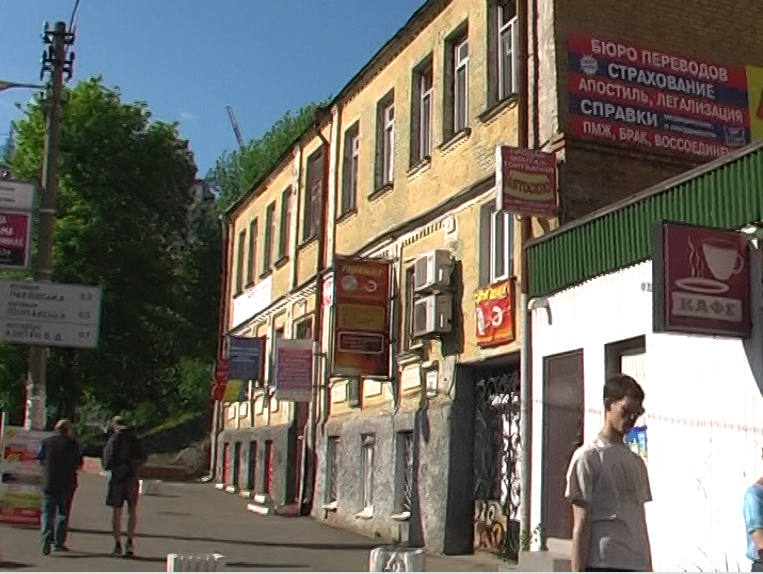
\includegraphics[width=\linewidth]{chast-vosp/musmags/moon-02.jpg}

\textit{2013 год, Рок-шоп. Кадр из фильма «Киевская амплитуда: Прогулка в прошлое».}
\end{center}

Доезжал до метро Универ, пешком спускался к цирку. Оттуда в обратном направлении топали патлатые рокеры в черном, с разными цепями, здоровенными перстнями, с повязанными на голове банданами. Они все шли с Володарского. 

На самой улице, которая отделяется от площади с цирком, рокеров и прочих неформалов было еще больше. Пахло табаком – еще работала разоренная ныне табачная фабрика, по левой стороне. Справа, кроме советской высотки номер 4, стояли старые дома, и за ними проглядывали просторные дворы и пустыри, а позади – снова старые дома уже на Дмитриевской. Вдалеке, между плодовыми деревьями были натянуты бечевки, сушилось белье. Потом было снова несколько домов новее, а Moon находился в желтом двухэтажном, давнем, у небольшого поворота. Под тридцатым номером.

Там в подвале был рок-шоп Core, а на втором – Moon, над входом, чуть правее двери. В Moon кассеты продавали только от Moon и дешевле, чем внизу, где торговали кроме «студийных» кассет еще и кустарными, записанными на 90-минутки. Попав в Moon впервые, я вообще не знал «роковую» направленность обоих магазинов. Я думал, это лавочка вроде Western Thunder с музыкой на любой вкус.

И вот я отворил высокую, обитую вагонкой дверь и попал в затхлое парадное. Четко знал, что надо на второй этаж – так было написано на обложке. Поднялся узкой лестницей, свернул направо.

Порог, открытая квадратная комната, довольно темно. Три стены – у двери, слева и справа – заняты стеллажами с кассетами, а впереди то ли за прилавком тоже с кассетами, то ли за столом – продавец. У продавца – магнитофон «Маяк». Продавцы сменялись. Был культурный – и советы давал, и кассеты не жлобился ставить, а был болтун матерщинник, вечно с кем-то из друзей стоял и перебрасывался новостями музыкального мира. Но забегаю вперед.

Сейчас я впервые в Moon, стою и разглядываю кассеты. Всё названия мне незнакомые, ибо продавался там большей частью такой рок, который даже по радио не звучал. Обложки с изображениями скелетов, живых мертвецов, волков, полуголых красавиц. В прямоугольничках пояснения, что за жанр: melodic black, gothic и тому подобное. Стояли неформального вида две девушки, тоже выбирали музыку.

Я долго бегал глазами от одной кассеты к другой, пока не спросил у продавца: «А что-нибудь электронное у вас есть?». Тот подумал и присоветовал группу Think About Mutation, альбом Hellraver – могу слушать его до сих пор кстати. Так начались мои посещения Moon. В Western Thunder я уже не ходил. То ли он к тому времени закрылся, то ли музыка в Moon показалась мне интереснее.

Сначала я таки высосал там всю электронику – два альбома Scorn, сборник Alternative World (где были Jarboe и Coil). Когда в Moon запасы электронной музыки иссякли, я спустился в подвал Core.

На подходах, в коридоре, все стены обклеены объявлениями. Такой-то группе нужен вокалист, а вот ударник с репетиционной базой ищет гитаристов, петь он может и сам. Много было просто вокалистов. Они указывали, каким голосом и манерой способны петь. «Могу гроулом».

Внутри за прилавком с кассетами стоял колоритный бородач. В Core я надыбал еще один альбом Scorn – Loggi Baroghi, и Green Nuns Of the Revolution – после чего переключился на рок.

Помимо кассет, продавались банданы, футболки, рюкзаки соответствующей тематики, а также напульсники с заклёпками, перстни с черепами и прочее, прочее. Всё это висело на стенах, лежало на полках и в стеклянных коробах.

Я скоро затащил сюда брата Сашу, и мы уже ходили оба в банданах – у Саши в крупных черепах, у меня в паутине и мелких черепах. Также я обзавелся рюкзаком с изображением зомби да надписью «Punks not dead» (именно так). Позже сменил его на Нирвану.

Музыку продолжал брать в основном этажом выше. Вернее, двумя.

Обычно я шел туда во второй половине дня – попасть после обеда. С собой брал плейер, чтобы на обратном пути насладиться новым альбомом. Покупал  кассету, ставил её на прослушивание и шел пешком дальше, к Лукьяше, мимо фабрики театрального реквизита и потом срезал угол через пустырь между Речной, частью Володарского и Косиора (ныне Черновола). На этом пустыре и вокруг него сейчас выросли огромные домины.

Четко помню с левой части пустыря убогое, вдохновляющее здание из потемневшего от времени кирпича, тесный дворик, зеленые заросли. Потом там затеялась вечная стройка, появился вагончик рабочих, но до возведения титанического жилого комплекса было далеко, и я ходил через пустырь даже когда его оградили зеленым деревянным забором.

В тех краях протекал некогда ручей Скоморох, местные называли его Лыбедью, а я ничего об этом не знал. У меня в наушниках звучала новая музыка, и я выруливал на улицу маршала Рыбалко, где шел вдоль копейной ограды стадиона «Старт», известного по «мачту смерти». Но для меня тогда это был просто безымянный стадион, и хотя мы с братом катались там пару раз на скэйтах и я наверняка видел памятник участникам этого матча, однако не придал этому значения. Меняется восприятие одних и тех же мест, теперь оно стало глубже, всякое место имеет историю, лишено сиюминутности.

\begin{center}

\includegraphics[width=\linewidth]{chast-vosp/musmags/00.jpg}

\textit{2005 год, я на фоне ограды «Старта».}
\end{center}

На другой стороне улицы, в одном из домов, на первом этаже, был пункт проката разной техники – телевизоров, магнитофонов. Не знаю, существуют ли сейчас такие пункты. У бабушки там работали знакомые, благодаря чему она купила задешево списанный телевизор и пару раздолбанных магнитофонов.

У перекрестка Рыбалко и Шолуденко – вход на стадион, состоящий из множества арок с воротами, за колоннадой. Там были написаны адреса узлов любительской сети Fidonet, популярной в 90-е и начале этого века. Несколько дальше, на улице Бердичевской, на бетонном заборе Лукьяновского трамвайного депо, виднелись рекламные граффити местного, киевского левонета, аналога Fidonet – X-Files Net.

\begin{center}
\includegraphics[width=\linewidth]{chast-vosp/musmags/\myimgprefix IMG_20140308_154056.jpg}

\textit{Март 2014. Улица Рыбалко.}
\end{center}

\begin{center}
\includegraphics[width=\linewidth]{chast-vosp/musmags/\myimgprefix IMG_20140308_154220.jpg}

\textit{Март 2014. Колоннада у входа на стадион.}
\end{center}

\newpage

Расскажу об этом подробнее. До эпохи распространения Интернета, отдельные энтузиасты, владельцы домашних компьютеров, заводили так называемые «бисы». BBS – Bulletin Board System – нечто вроде сайта, но вне интернета. При помощи подключенного к телефонной сети модема и программы-терминала, вы звонили по номеру обычного городского телефона на «бису». Соединение. Вы попадали в текстовый интерфейс. В зависимости от программного обеспечения и желаний владельцев «бис», предоставлялись разные файлы для скачивания, иногда почта в рамках самой бисы, порой нечто вроде простеньких форумов. 

Телефоны «бис» встречались на фонарных столбах, стенах домов. Некоторые компьютерные фирмы держали свои «бисы» и публиковали о них сведения в журналах. То ли на Щусева, то ли на Вавиловых была одна такая...
 
Наряду с бисами развивался Fidonet и другие сети на основе FTN-технологии. Состоит она вот в чем. Сеть использует телефонную линию для передачи данных. Кстати, тарификация тогда была советской, то есть абонплату вносишь и пользуйся телефоном сколько влезет. Позже, введение поминутки нанесло Fidonet'у удар.

Сеть состояла из узлов – «нодов», и подключенных к ним точек – «поинтов». Ноды отвечали за передачу данных между собой, согласно определенной договоренности, в назначенное время. Сетью предоставлялся, по сути, набор форумов, или эхо-конференций, а также почта и возможность скачивать с нодов файлы, что называлось «фреканьем» (от file request, запрос файла). Существовало понятие «фидошного софта» и «набора поинта». Последний включал в себя программы, нужные для того, чтобы общаться в сети.

А именно. Редактор «Голый дед», вернее GoldEd – для работы с почтой и сообщениями в эхах. Программа-тоссер – для управления базой данных сообщений. «Тимыло» (t-mail) – программа для приема и передачи данных, подготовленных тоссером. Вы запускали тимыло и прозванивались к ноде, за которой были закреплены. Тимыло отправляло написанные вами сообщения, скачивало новые, запускало тоссер для их распаковки. Затем вы открывали Голого деда и читали в нем сообщения. Писали  новые, снова запускали тимыло и прозванивались к ноде. 

Всё это работало на энтузиазме и потом заглохло. Сейчас Fidonet существует в узком кругу старых фидошников, задействуя для передачи данных Интернет.

Fidonet охватывал, по сути, весь мир, и страны бывшего Союза в частности. В Киеве возникли местные, чисто городские «левонеты», основанные на той же технологии, что Fido. Припоминаю X-Files Net, и сеть компьютерных музыкантов (большей частью трекерщиков) DreamNet, которая распалась, когда основатель сети продал свой компьютер. Я участвовал в Fidonet и Dreamnet.

А теперь вернусь к музыкальным магазинам! И я еще не дошел до Лукьяши! Я только поворачиваю вдоль стадиона, по улице Шолуденко, в сторону предприятия Газприбор. У проходной стояли щиты с фотографиями заводской базы отдыха, кажется на реке Рось.

У многих предприятий были свои, ведомственные базы отдыха, куда рабочих по путевкам отвозил автобус. 

Моя бабушка Таня работала на Полиграфкниге, которой принадлежал лагерь отдыха «Бережок», на берегу Десны. И вот в назначенный день, летним утром, за каждой семьей, у которой была путевка, прямо к дому приезжал небольшой автобус с Полиграфкниги. Собирал всех, и ехал через дамбу Киевского водохранилища в сторону Чернигова. 

От Полиграфкниги, этой крупнейшей типографии, ныне осталась разве что проходная. Цеха  расформированы, помещения отданы в аренду. А раньше, что ни книжка украинского издательства, то на последней странице – адрес Полиграфкниги, улица Довженко 3.

На другой стороне улицы Шолуденко, против Газприбора, там где теперь два здания налоговиков, стояли общаги. Одну отреставрировали и оставили как есть, а вместо зеркального небоскреба был пустырь, либо другая общага, не помню.

Перекресток на улицу Бердичевскую, прежде – Белорусская площадь. Я сворачивал на Бердичевскую, между больницей и бетонным забором Лукьяновского трамвайного депо. Оно еще работало, там жили и чинились трамваи. Бердичевская всегда представляется мне в сумраке. С фиолетового декабрьского неба, через подсвеченный желтыми фонарями туман, валит мокрый снег.

Можно было завернуть к бабушке, или сразу ехать домой, на Бастионную, с новой музыкой в ушах – я выходил со станции метро «Дружбы народов», спускался от Печерского моста и всё время видел впереди свой, стоящий на холму, дом – издалека он казался крепостью, замком, довлеющим на окрестностями.

Шло время, я посещал рок-шоп всё реже. 

Сгинул магазин «Moon» – сначала он вроде бы переехал ближе к вокзалу, а когда я туда добрался, он вовсе закрылся. 

Я тоже переселился, но по старой памяти ездил в «Core», покупал диски – у меня появился компьютер, а эра кассет отошла в прошлое. Приобрел однажды альбом группы Defecation, по стилю нечто вроде grindcore. Зашел потом к бабушке. Брата дома не было. Говорю, хочу диск проверить. Поставил в музыкальный центр, играет песня. Бабушка слушала-слушала, потом спрашивает – когда же начнется музыка?
  
Никогда не фотографировал здание рок-шопа, всё думал – оно будет стоять вечно, никто не тронет, зачем? Дважды снимал его на видео – в фильме «Калейдоскоп» (2005) есть сцена про рок-шоп, и в «Киевская амплитуда: Прогулка в прошлое» 2013 года мы подошли к нему, он был закрыт, но запечатлели со всех сторон его и окрестности, задворки.

И вот в марте 2014-го, я отправился проведать знакомые места, заодно сделать снимок желтого домика для этой книги. 

Вместо чтоб идти по Володарского, уже Златоустовской, сделал крюк через Дмитриевскую, свернул на Павловскую, вернулся чуть назад – поэтому не видел издали, как если бы изначально шел от цирка по Володарского. И тут поразило! Нет больше рок-шопа.

\begin{center}
\includegraphics[width=\linewidth]{chast-vosp/musmags/\myimgprefix IMG_20140308_152805.jpg}

\textit{Март 2014. Здесь был рок-шоп.}
\end{center}

\begin{center}
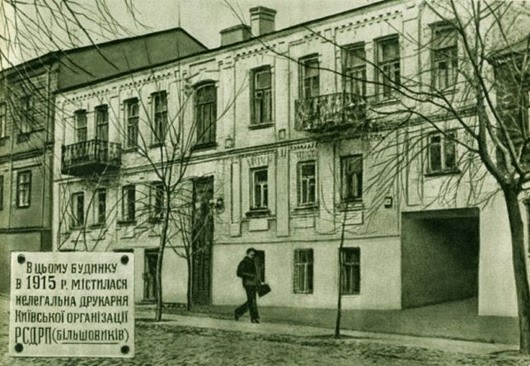
\includegraphics[width=\linewidth]{chast-vosp/musmags/rock-50.jpg}

\textit{А так выглядел дом рок-шопа в 1950-х.}
\end{center}

\newpage

Да, конечно, сам магазин переехал на Петровку, но мне какое дело? Важна была улица, и дом на ней, и воспоминания, оживающие каждый раз при посещении. А теперь только и осталось, что  воспоминания. И незачем мне больше ходить сюда!

В девяностые, было еще два рок-шопа. Это «Домино» – во глубинах за Пассажем, в опять-таки полуподвальном помещении, на одной из улиц – Заньковецкой, Городецкого, Ольгинской, точно не помню. Он давно исчез. Весь магазин располагался в длиннющем коридоре, тупиком упираясь в витрину с кассетами. По стенам висели товары – рюкзаки, футболки. Это если свернуть от входа справа. А слева – еще одна лавочка чисто с рюкзаками? Вроде да.

Другой рок-шоп, внутри я не был, только проходил мимо, а потом его закрыли. Возле станции метро «Кловская», назывался «Перекресток», на улице Первомайского или на Печерском спуске? Тоже в подвале.

Теперь уже невозможно снова пережить те ощущения, которые возникали от поездки к черту на Кулички за кассетой. Сейчас захотел – скачал альбом. Захотел – скачал тысячу альбомов. Не вставая со стула. Простое желание просто исполняется. В книге воспоминаний про Шукшина один режиссер мечтал – а хорошо бы иметь дома фильмотеку! Технически это стало возможным. Носи себе в кармане фильмы, библиотеку, фонотеку. Однако эта дармовщина и доступность некоторым образом обесценили произведения искусства.

Так ты заранее готовился, выделял время на поездку в рок-шоп. Черт знает, что там интересного найдешь? Денег есть, скажем, на две кассеты. Сами эти носители – материальные предметы, в коробочках, от которых пахнет новой пластмассой и бумагой обложки. Кассету можно пальцем покрутить, поглядеть сквозь прозрачный корпус на пленку – а сначала там идет светлый шероховатый отрезок, для чистки магнитофонных головок. Ты смотришь пленку и понимаешь – там записана музыка. Ты держишь её в руках.

Я хранил кассеты в ящиках письменного стола. У меня там лежали кассеты и картриджи к игровой приставке «Денди». Кассеты я расставлял по сериям и по тому, какие чаще слушал. Самые хреновые запихивал подальше. На осень 1997 года я собрал 150 кассет, и пополнял фонотеку еще несколько лет, пока постепенно не перешел на диски и MP3.

Покупка кассеты была событием, осмысленным времяпровождением, как и покупка книги – поэтому я в целом помню, где брал каждый альбом или книгу. Поскольку кассеты в фонотеке, в отличие от файлов, имеют конечное количество, то они многократно переслушивались. 

Скажу иначе – альбом на кассете слушался чаще, чем теперь такой же альбом в электронном виде. Сейчас у тебя заведомо шире выбор. Но странная штука – вроде и так, но количество хорошей музыки, попадающей мне в руки, на кассетах было выше. Что ни альбом или сборник – в точку! Фуфло попадалось редко. Сегодня же ищу, чего бы скачать, сотни альбомов проклацаю по паре песен – нечего слушать, однообразно всё и обыкновенно.

Время от времени продажу пиратских кассет запрещали. Тогда исчезали уличные раскладки. Но не только! Так, после сурового запрета от 1 января 1998 года, я ломанулся к Western Thunder, потом, спустившись по Воровского к цирку, в Moon – везде было закрыто. Но эдак через месяц, кассетами снова торговали.

Какие еще были музыкальные магазины в девяностых годах?

«Два меломана» на Петровке. Продолговатый киоск этот стоял на пути к зданию по адресу Вербная 16-А, сразу за зданием номер 14, если идти от выхода из метро, что ближе к книжному рынку. Но удобнее было покинуть станцию через северный выход и сразу свернуть на восток.

В «Двух меломанах» почти не торговали атрибутикой. Зато продавали самую разную музыку, много редкой электроники и, как тогда говорили, альтернативу. Из рока всё, что считалось недостаточно тяжелым для Moon и Core, можно было найти здесь. От Нирваны от Сепултуры.

Вход в магазин был слева, оклеенная каким-то скотчем дверь на приступочке, зимой вечно скользкой, так что приходилось держаться, чтобы не упасть. Внутри тесно, не развернуться. Ларек просуществовал до 2007 года, потом на его месте открыли гендэлык. В 2016-м, «Два меломана» обретаются на самом книжном рынке Петровка и держат интернет-магазин.

Кстати студия Moon, в отличие от славного магазина, тоже здравствует, переметнулась на выпуск популярной музыки и находится в тихом райончике неподалеку от Караваевых дач, в пятиэтажке на улице Искровской.

Магазин в КПИ. В девятом или двадцатом корпусе. Навскидку не помню, а пилить туда нарочно смотреть и уточнять – не с руки. Раньше я много ездил на радиорынок, на Кардачи. Точнее, ходил туда пешком от метро Политех или от Большевика. И вот по пути от Политеха, если свернуть в один из корпусов налево, был этот музыкальный магазин. На первом этаже, отгороженный от холла. Я отоваривался там раза четыре, брал электронную музыку – на самопальной кассете, альбом транса Freaky Chakra, сборник «Tantrance», потом, занудный Ultrabass, и в коричневой обложке Banco de Gaia.

Самые приятные воспоминания у меня остались от посещений Western Thunder в здравствующем тогда Сенном рынке, да желтого домика на Володарского. Ничего этого больше нет.

Где-то там в прошлом на склонах Днепра осталась, забываясь, Зеленка\footnote{На 2017 год, в полусотне метрах к северо-западу от Зеленки есть ресторан «Курени», и там деревянный дом. По 1965-й, на Козловской, 2, в нем жило четыре семьи. Вся усадьба, занимаемая ныне рестораном, по 1957 год была частным владением, подаренным участнику 1-й Мировой войны Лаврику за заслуги перед Отечеством. В 1965-м жильцов отселили и военные содержали там арестантов, поставив на окна решетки.} – в самом деле, как любая заброшка, заросшая зеленью. Зеленый Театр. В 1950-х – переделанное под эстраду и кинотеатр военное сооружение 19 века. В девяностых на его пустынных развалинах, исписанных названиями музыкальных групп вроде Нирваны, собирались неформалы, тогда же зарождалось и диггерство. Я обхожу вниманием связанные с Зеленкой мистические байки о Хозяине, случаях безумия, каких-то порталах и прочем.

%На стенах Зеленки пестрели названия групп вроде Nirvana, а про тамошние и окрестности подземелья ходили мистические легенды. Говорили про некоего Хозяина, загадочного хранителя Зеленки – конечно же, одетого в длинный плащ, с лицом, сокрытым под капюшоном. О подземельях же баили, будто там расположены порталы в параллельный мир.

К Зеленке подбиралась цивилизация, новые поколения нефоров облюбовали уже деревянную лестницу на БЖ, Большой Житомирской, в конце Десятинного переулка. Раньше эта лестница была красивая, каменная, вела в жилой район урочища Гончары. В 2016 году деревянную лестницу принялись реконструировать.

С середины нулевых неформалы и оттуда сгинули, переселившись на форумы да в социальные сети. Перед этим уходом в электронный мир их еще можно было заметить на лавочках за Филармонией, на подходах к Арке Дружбы народов.

Ныне, представители сего подвида рода человеческого, иногда встречаются на зверинецкой Лысой горе и в ея окрестностях.
